\documentclass[../main.tex]{subfiles}
\graphicspath{{\subfix{../media/}}}


\begin{document}
	
	\par Anther extension to the concept of integration is computing of the integration of a mathematical form\footnote{function} along a curve. This operation is called line integration.
	\begin{definition}
			Line integration of a mathematical form $\mathbf{F}$ is a the cumulative change of $\mathbf{F}$ along a path defined by some curve $C$ 
	\end{definition}
	
	\par As for its computation; inherited from general idea of integration, line integral exploit the concept of Riemann summation in its evaluation of the integral. This is done with the following steps:
	\begin{enumerate}
		\item Divid the curve $C$ to $n$ small subarcs\footnote{small arcs} $\Delta s_1, \dots \Delta s_n$, see figure \ref{fig: parametric curve}.
		\item For every subarc $i$, evaluate the mathematical form $\mathbf{F}$ at some point\footnote{choice of $P_i^*$ will decide which Riemann sum we have. Either Right, Left, Midpoint Riemann sum} $P_i^* \in \Delta s_i$.
		\item Compute $\mathbf{F}(P_i^*) \Delta s_i$ for every subarc "i.e the area of a rectangle with length $\mathbf{F}(P_i^*)$ and width $\Delta s_i$ for subarc $i$".
		\item Sum the rectangles to approximate the area under $\mathbf{F}$ along path $C$.
	\end{enumerate} 
	
	\par Hence you have the general form of line integration of $\mathbf{F}$ along a path defined by some curve $C$
	\begin{equation}
		\int_C \mathbf{F} ds = \lim_{n \rightarrow \infty} \sum_{i=1}^n \mathbf{F}(P_i^*) \Delta s_i 
	\end{equation}
 	
 	\par The following figure illustrate step 1 of computing the line integration of a mathematical form $\mathbf{F}$, which is dividing the curve $C$ into subarcs $\Delta s$.
	\begin{figure}[h]
		\centering
		\begin{tikzpicture}[
				declare function={
					xs(\t) = 6*\t*cos(deg(5*\t));
					ys(\t) = 6*\t^3 - 6;
					}
				]
			\begin{axis}[
			  	view={0}{90}, % for a view 'from above'
			  	domain=-7:7,
  			    xmin=-7, xmax=7,
			    ymin=-7, ymax=7,
	  	        width=0.5\linewidth
				]
				\addplot[thick, samples=20, parametricmarker, samples y=0, domain=0.5:1.1, variable=\t] ({xs(\t)}, {ys(\t)});
				
				\addplot[red, thick, samples=3, samples y=0, domain=0.891:0.96, variable=\t] ({xs(\t)}, {ys(\t)});
				\node at (axis cs:0.5,0.8) [red, anchor=north east] {$\Delta s_i$};
			\end{axis}
		\end{tikzpicture}
		\caption{Dividing curve $C$ in to subarcs $\Delta s$}
		\label{fig: parametric curve}	
	\end{figure}

	\par As for the mathematical forms that we will address in this script, are scalar valued functions in $\mathbb{R}^2, \; \mathbb{R}^3$ and  vector fields in $\mathbb{R}^2, \; \mathbb{R}^3$

	\newpage
	\subsection{Scalar Function}
		Let $f: \mathbb{R}^k \rightarrow \mathbb{R}$ a scalar valued function that maps set 
		\begin{definition}
			Line integration of a scalar valued function $f(\mathbf{x})$ along a smooth curve $C$
			\begin{equation}
				\int_C f(\mathbf{x}) ds = \lim_{n \rightarrow \infty} \sum_{i=1}^n f(\mathbf{x}_i^*) \Delta s_i 
			\end{equation}
		\end{definition}
		
		\begin{example}
			Given a scalar valued function $f(x, y) = 0.6\cos \left ( \sqrt{x^2+y^2} \right ) + 3$ and a parametric curve $C$ defined by following equations 
			\begin{align*}
				x &= 6t \cos(5t)		&&y = 6t^3 - 6\\
			\end{align*}
			,or equivalently by vector equation $r(t) = 6t \cos(5t) \; \mathbf{i} + (6t^3 - 6) \; \mathbf{j}$; graph the Riemann sum approximation of the line integration of $f(x, y)$ along curve $C$ for arbitrary $n$
		\end{example}
		\begin{solution}
			For arbitrary chosen $n$, that is not too large; the Riemann sum would look rectangles that cover the area between curve $C$ and function $f(x,y)$.
			
			\begin{figure*}[h!]
				\centering
				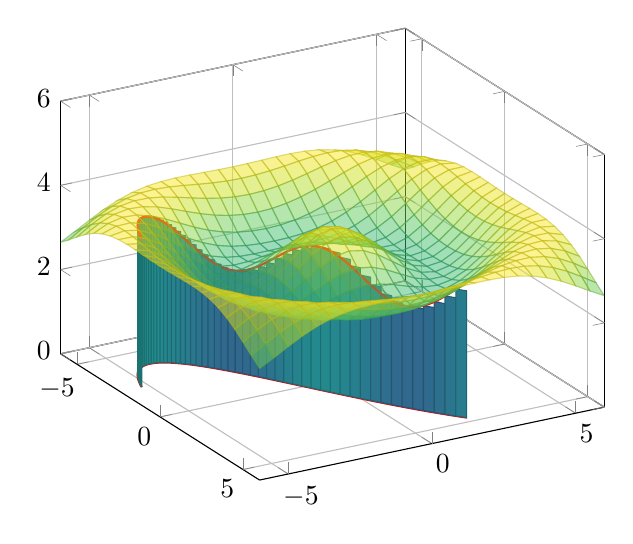
\begin{tikzpicture}[
					declare function={
						f(\x,\y) = 0.6*cos(deg(sqrt(\x^2+\y^2))) + 3;
						xs(\t) = 6*\t*cos(deg(5*\t));
						ys(\t) = 6*\t^3 - 6;
						}
					]
				    \begin{axis}[
				        view={60}{30},
				        grid=both,
				        colormap/viridis,
				        domain=-6:6,
					    xmin=-6, xmax=6,
				        ymin=-6, ymax=6,
					    zmin=0, zmax=6,
					    width=0.7\linewidth,
					    ]
					    
					    % parametars
					    \newcommand{\h}{0.01}
	
						% parametric curve in (x,y,0) plane
						\addplot3 [red, thick, samples=100, samples y=0, domain=0.5:1.1, variable=\t] ({xs(\t)}, {ys(\t)}, 0);						
						\pgfplotsinvokeforeach{0.5,0.5+\h,...,1.1-\h}{
		    					\addplot3 [red, patch, patch type = rectangle] coordinates {
									({xs(#1)}, {ys(#1)}, 0) 
									({xs(#1+\h)}, {ys(#1+\h)}, 0) 
									({xs(#1+\h)}, {ys(#1+\h)}, {f(xs(#1),ys(#1))}) 
									({xs(#1)}, {ys(#1)}, {f(xs(#1),ys(#1))})
									};
						}
						\addplot3 [red, thick, samples=100, samples y=0, domain=0.5:1.1, variable=\t, point meta=0] ({xs(\t)}, {ys(\t)}, {f(xs(\t), ys(\t))});
												
						% function
						\addplot3 [surf, opacity=0.5] {f(\x,\y)};	
						
				    \end{axis}
				\end{tikzpicture}
			\end{figure*}
			The plot above is the approximated line integration of $f(x,y)$ along curve $C$ using Riemann sum.
		\end{solution}

		
	\subsection{Vector Function}
	
		\begin{figure}[h]
			\centering
			\begin{tikzpicture}[
					declare function={
						xs(\t) = 6*\t*cos(deg(5*\t));
						ys(\t) = 6*\t^3 - 6;
						}
					]
				\begin{axis}[
				  	view={0}{90}, % for a view 'from above'
				  	domain=-7:7,
	  			    xmin=-7, xmax=7,
				    ymin=-7, ymax=7,
		  	        width=0.5\linewidth
					]
					\addplot3[point meta={sqrt((2*x*y)^2 + (x^2 - 3*y^2)^2)}, quiver={u=2*x*y, v=x^2 - 3*y^2, scale arrows=0.01, every arrow/.append style={-{Stealth[scale=0.2+0.8*\pgfplotspointmetatransformed/1000]}}}, samples=17] (x,y,0);	
					
					\addplot[red, thick, samples=20, parametricmarker, samples y=0, domain=0.5:1.1, variable=\t] ({xs(\t)}, {ys(\t)});
					\addplot [|->, thick,  black] coordinates { (0,0) (3,1)};
				\end{axis}
			\end{tikzpicture}
			\caption{Dividing curve $C$ in to subarcs $\Delta s$}
			\label{fig: parametric curve}	
		\end{figure}
	
\end{document}